\documentclass[ebook,10pt]{memoir}
\usepackage[version=3]{mhchem}
\usepackage{fourier}
\usepackage{graphicx}

% Page style: headers, footers, &c.
\setlength{\headwidth}{\textwidth}
\addtolength{\headwidth}{\marginparsep}
\addtolength{\headwidth}{\marginparwidth}

\makepagestyle{narbonic}
  \makerunningwidth{narbonic}{\headwidth}
  \makeevenhead{narbonic}{\theauthor}{}{}
  \makeevenfoot{narbonic}{\thepage}{}{}

  \makeoddhead{narbonic}{}{}{\thetitle}
  \makeoddfoot{narbonic}{}{}{\thepage}

% Special style for the first page of the story; since we want to 
% suppress the headers on the first page.
\copypagestyle{narbonicfirst}{narbonic}
  \makeevenhead{narbonicfirst}{}{}{}
  \makeoddhead{narbonicfirst}{}{}{}

% This makes the line filling better-- \fussy leaves us with too 
% many overhanging lines.
\midsloppy

%% Meta
\title{A Killer Pesto}
\author{Shaenon K. Garrity}
\date{}

%% Apparently deep magic here; must be last?
\usepackage[pdftex]{hyperref}
\hypersetup{colorlinks,%
	citecolor=black,%
	filecolor=black,%
	linkcolor=black,%
	urlcolor=black,%
	pdftex}

\begin{document}

\frontmatter 

\pagestyle{empty}
\vspace*{\droptitle}
\begin{flushright}
\Huge \thetitle

\Large The Narbonic Filename Story

\vspace*{20em}
\large \theauthor

\end{flushright}
\newpage

\begin{center}
\vspace*{20em}
All rights reserved.

Copyright \copyright{} 2011 Shaenon K. Garrity
\end{center}

\newpage
\begin{center}
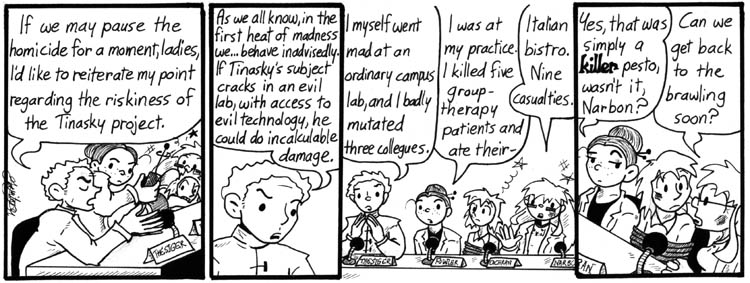
\includegraphics{killer_pesto}
\end{center}

\vspace*{5em}
\small
This story was originally published as a serial, from November 12th,
2002 until August 30th, 2009, in the file names of the images
comprising the web comic \emph{Narbonic}. Due to the limitations of
the medium, the story was published a few words a time, and was
originally published without punctuation. An official version has
never been released by the author, and so it has been left to fans to
reconstruct.

This version is based on the version hosted by John Campbell at 
\mbox{\href{http://www.ci-n.com/~jcampbel/narbonic.txt}{http://www.ci-n.com/$\sim$jcampbel/narbonic.txt}}.
In the absence of any canonical version, the punctuation and 
capitalization has been cleaned up in accordance with my own tastes.
Therefore, if you find any fault in the story, the blame should be 
placed squarely at my feet.

\vspace*{4em}
John Doty

May 29th, 2011

\cleardoublepage



\mainmatter
\normalsize
\pagestyle{narbonic}
\thispagestyle{narbonicfirst}

When Octavius Winter told people---normal people---that he was an evil
attorney, they always responded with some jolly variant on ``Aren't
they all?''

Winter had a special gaze reserved for those people. It was on the
surface almost identical to his usual cold grim workaday glare, the
only discernable difference was that it inspired the target to
instantly stagger back, gibber an apology, or burst into
tears---generally all three.

He was an evil attorney. Like only the best evil attorneys, he knew
that his clients (whether world-conquering despots, twitchy mad
scientists or the slick and reptilian heads of sinister corporations)
appreciated a modicum of the appropriate style from the henchmen and
servitors in their hire. For a lawyer, this meant a complexion of
fungal sallowness, a dour visage carved in deep and portentous lines,
hair slicked back from a widows peak, expensive dark suit with
shoulders broad enough to accommodate a brace of vultures and,
whenever possible, a cloak. The gaze was just the maraschino cherry on
the macabre hot-fudge sundae of Octavius Winter, Evil Attorney at Law.

For what he charged, it was the least he could do. Evil law was
steady, rewarding work. Winter's practice attracted the types of
clients who had plenty of liquid cash, suffered frequent difficulties
with the law and were generous in their peculiar way to those willing
to help them. Villains are a lawyers dream. 

Winter did get the occasional bad apple, one of those shortsighted
would-be overlords who try to murder their own hirelings, up to and
including licensed legal representatives, simply to prove their
ruthlessness, but it was for just such frivolous individuals that
odorless poisons had been developed, after all.

Winter didn't much mind handling the bad apples in the evil
community. He always politely but firmly requested payment up
front. Yet the functions of an evil attorney do include some genuine
unpleasantness and Winter, as his tasteful black sedan slid through
the shadows of the university's sunny tree-lined drive, suspected that
he might be approaching some of it.

He was not pleased. 

True, the Narbon estate was in many respects the finest entry in his
impeccable portfolio and he was willing to endure much for it. Before
Dr. Helen Narbon had hired Winter, her family's legal affairs had been
handled for uncounted generations by Elijah Threadham, one of the true
legends.

Winter remembered reading with boyish awe in his days as an amoral law
student of how the mere entrance of the venerable lawyer into a
courtroom, stapled-together flesh dripping and eye sockets emitting
their familiar red LED glow, had won the Narbon family many hasty and
agreeable out-of-court settlements. When Threadham had at last gone
irrevocably to pieces and Dr. Narbon had reluctantly stopped digging
him up and hooking him to the galvanizer for one last case, Winter had
been honored to assume the position of the Narbon's new attorney.

But that had been many years ago, when Dr. Narbon was an ambitious
young mad scientist with a string of zombie-related lawsuits still
ahead of her. Winter had liked Dr. Narbon as much as he liked
anything. He would miss her nasty, brutish, and consummately
professional business demeanor. He knew only two things about the
younger Helen Narbon, the girl with whom he was about to deal: she was
old enough to sign legally binding documents, and she was sane. The
first point made his job much easier. The second, he reluctantly
admitted in the clammy depths of his heart, worried him.

Well, this was her dormitory. Time to protect the Narbon interests.

Gamine coeds in undersized T-shirts idled in the sunshine outside the
ivy-dappled building, smoking slim cigarettes and listening to
bubblegum on a portable radio. Winter descended on the tableau like
the bad fairy storming the enchanted palace, freezing the girls
mid-smoke. He carried a black leather attach\'{e} case in one hand and
a bone-handled walking stick in the other, and he was the worst thing
they had ever seen. The radio actually fell silent as he passed.

A good entrance was the backbone of an evil attorney's courtroom
work. It was hardly to his credit that so few of his colleagues
rehearsed as conscientiously, or took tradition as seriously. When,
however, the plump woman behind the desk in the lobby fell backwards
over her chair in her panic to scurry away from him, then lay on the
floor like a pastel beetle with her round legs kicking helplessly at
the air, the corners of Winter's colorless lips did turn briefly,
incrementally upwards before he remembered himself.

He loomed over the desk. ``I am looking,'' he intoned (thanks to years
of careful practice, it was difficult for Winter not to intone) ``for
a Helen Narbon.''

The desk attendant popped into a sitting position. Her face glowed
with the relief of someone who has just been informed that the bell
tolls not for her, but just for old Quasimodo again.

``Oh, oh, her. I---I think she's waiting for you in the common room.''
She pointed eagerly down the hall, her arm quivering.

The common room, Winter reflected with distaste, was as brainlessly
pleasant as the rest of the campus: rose draperies, fuzzy armchairs, a
few abandoned textbooks fading in the late-afternoon sun. The whole
place was a round-bellied puppy begging to be kicked.

Dr. Narbon would never have been seen dead (or undead) in a place like
this. She had of course occasionally lectured at colleges; usually in
the dead of night, usually in an institution with Invisible, Arcane or
possibly Enochian in its title. This was not the same thing at
all. And meanwhile, the younger Helen Narbon, having abandoned her
familial responsibilities seven years past, the sole inhabitant of the
parlor, was curled in a burgundy armchair, her back to the door.

Winter loomed forward to investigate. The girl's blonde ponytail swung
over the open pages of the textbook, casting pink shadows over complex
biological diagrams which Winter, had he been asked, could neither
have identified nor feigned any interest in.

Winter was not in the habit of making polite noises to introduce
himself for much the same reason a tiger on the stalk is not in the
habit of clearing its throat. ``Helen Beta Narbon,'' he demanded.

The girl jumped, then turned to face him.

Winter chided himself for the chill that ran up his spine. He had,
after all, expected this. The Narbons were mad scientists all the way
down their makeshift line. Winter had only the mildest interest in
what his clients did with their time when they weren't being clients,
but he was vaguely aware that mad scientists had their
specialties. Professor Caesar controlled the weather, Lupin Madblood
and Felix Madblood before him were killer-robot men, Madame Onyx had
been into particle physics before vanishing into that parallel
dimension. (Unfortunate business, she still owed him a retainer from
the vanishing-island settlement.)

The Helen Narbons were biologists. Reviving the dead was a talent of
theirs. So was engineering beast-men. So was cloning. It was how they
made more Helen Narbons. It was hard to picture them going through the
usual biological channels. Winter should not have been startled then
that Helen Beta was a photocopy of Dr. Narbon at twenty-five: the age
lines erased from the round apple-cheeked face, the calculating gleam
wiped from the large blue eyes. He should not have been startled, and
was deeply disappointed in himself for it, but he was. In the course
of his career Winter had seen the dead rise from the grave, usually
smelling awful and angrily demanding personal-injury suits, but not
like this. This was eerie.

Helen Beta gazed wide-eyed into the long grim face of Octavius Winter,
a face that made strong men whimper when it frowned and shriek when it
smiled. Her brow puckered. ``You're one of Mom's people aren't you?
You've got the look.''

Winter inclined his head. ``I am, among other things, Dr. Narbon's
attorney and executor. You received my letter?''

``That's right. Why did you want to see me? And what happened to
Mr. Threadham?''

``Elijah Threadham died not long after you ceased communications with
Dr. Narbon.''

``He was already dead.''

``This time it took.''

``Oh.'' Helen frowned. ``Well, I don't know what Mom told you, but we
went over this with Mr. Threadham. She doesn't have any control over
me. It doesn't matter that I was created as an experiment. She
can't---''

``I fear you misunderstand the situation, Miss Narbon. Do you know of
a decent Italian restaurant?''

``What?''

``I prefer to discuss matters of a sensitive nature over
dinner. Unless you would prefer a more private venue?''

``Sensitive? Look Mr., was it, Winter?''

``Winter.''

``Mister Winter I cut my ties to Mom and her thingies when I left
home. I'm putting myself through college. I'm working toward my
doctorate.''

``In biochemistry, as I recall.''

``Lots of people study biochemistry. Lots of people are good at it. It
doesn't mean anything. And when I graduate this spring without blowing
anything up, without unleashing any horror, without tampering in god's
domain even a tiny little bit, I will find a nice job doing something
nice that helps people. You understand, I'm out of the family
business. I don't care what horrible thing Mom has done this time, and
I'm not bailing her out again.''

``Miss Narbon, you are the most recent in the long line of Narbon
women---''

``Immaterial.''

``---and as such you have certain legal responsibilities. Dinner?''

Helen deflated. It was as Winter had, with distaste,
suspected. Underneath a thin, brittle coating of bluster the girl was
pure marshmallow.

``Okay. Fine. Let's go.''

Helen stuffed her textbook into a lilac backpack and stood. She was
wearing a pretty pink blouse. This struck Winter as particularly
obscene. How dare this girl dress Dr. Helen Narbon's body in a pretty
pink blouse? It had tiny hearts embroidered around the collar.

Winters small sour stomach turned.

The radio on the front lawn had resumed normal play, the bucolic
sorority tableau was restored. As Winter, Helen bobbing nervously in
his wake, passed the college girls his ears picked up hisses of
conversation.

``Oh surprise, it's her again.''

``What do you think they got her for this time?''

``Hope she's not coming back.''

He flicked a glance at them. This time the radio exploded. 

``You don't seem well-liked here,'' said Winter, casting about for
light conversation.

``Oh, those girls.'' Helen tossed her head. ``There were
accidents. Early on. Some people will believe all kinds of rumors.''

``But you're much better now, I imagine.''

``Yes.''

``I'm sure you've never even laid a finger on those particular young
women.''

``Exactly.''

``And it didn't so much as occur to you how very easy it would be to
convert their bones to some highly corrosive acid which would eat
their soft young flesh from the inside out?''

``I'm much better.''

Now that Winter had time to reflect he saw that the really remarkable
thing about Helen Beta, all things considered, was how much she didn't
resemble her creator. Dr. Narbon's shock of dandelion hair had stuck
out from her head in the mad scientists regulation
finger-in-the-lightsocket formation with the odd clump burned or
bitten off. Helen's was bound back in a tight neat ponytail with a
stiffness that suggested too much styling gel, or perhaps wood
glue. Dr. Narbon's electric blue eyes had flickered behind a
formidable pair of black-framed Army-issue BCDs. Helen also wore
glasses, of course, but hers were fanciful little loops of filigree
perched on her nose as if ready to bail out at the first sign of
trouble. If it were possible for glasses to make a person look less
intelligent, these were the frames. And Helen hunched (something
Winter considered only acceptable for licensed hunchbacks), and chewed
her lip, and worried her brow. And that teeny-tiny voice\ldots

``Mr. Winter?''

Winter sighed. ``Miss Narbon?''

``Are you going to tell me what this is about?''

``Over dinner, Miss Narbon. I am very sorely in need of dinner.''

\pfbreak

Twenty minutes later, Octavius Winter was glowering. 

He seldom felt called upon to glower. His normal expression was more
than foreboding enough to communicate his disapproval, often across
state lines. The very fact that circumstances had gotten bad enough to
require a full glower was enough to dampen his already
thoroughly-mildewed mood.

``This is a nice place,'' said Helen Beta bouncing in her seat a little.

Winter allowed his gaze to travel slowly and witheringly around the
room. He was not accustomed to dining in well-lit establishments, and
the very fact that he could see his surroundings was enough to make
him dislike them. His dark little avian eyes squinted into the flat
fluorescent light.

``There is,'' he intoned, ``a jukebox.''

``It's a perfectly nice bistro,'' Helen said defensively, ducking
behind her laminated menu.

It occurred to Winter that the glower had relatively little effect on
his dining companion. She might be a damp little ball of pink fluff,
he reminded himself, but she had been raised by Dr. Narbon. Evil
probably didn't bother her that much. More likely it just made her
faintly homesick.

He allowed his face to realign itself along its well-worn grooves and
glanced down at the table. His aching eyes gazed blearily at artifacts
he found utterly alien and horrific: paper napkins, fiberglass
surfaces, little foil-wrapped pats of butter and a little sign urging
cheerfully ``ask you're server for our daily specials!'' Enough was
enough.

``To business,'' said Winter. ``Your mother is dead.''

Helen stared blankly. ``What?''

``Your mother, dead.'' Winter squinted crosswise at the menu as if
trying to avoid direct eye contact with it. ``Do you imagine they know
anything whatsoever about tortellini?''

``What do you mean, dead?''

Winter glanced up. ``You're a biologist aren't you? Now, as her
executor I have certain duties at this time, as do you as her heir.''
His attach\'{e} case snapped open. ``There is, to begin, some
paperwork to be signed.''

``Wait, what?'' Helen shook herself. ``How---how did she die?''

``Angry mob, I am assured. It was slow and agonizing.'' A rare blush
of human feeling moved Winter to attempt a consoling word or
two. ``She would have wanted it that way.''

``You ready to order?'' snapped a waitress.

Winter returned to his paperwork. ``I will have whichever of your a la
carte items is least tasteless. Do not under any circumstances bring
me anything you people consider wine.''

Helen rubbed her forehead. ``He'll have the tortellini. Bring me the
special and beer.''

As soon as the waitress was gone, Helen turned on Winter. ``Mr. Winter,
I don't appreciate this. My mother is not dead.''

Winter didn't answer. He could see no particular point. Two
gold-tipped pens emerged from his attach\'{e} case and took their
place at the table flanking Dr. Narbon's last will and testament.

``She's not,'' said Helen, her voice strained. ``She's got you
fooled. She's played dead any number of times. Don't you know that?''

From the depths of the case winter unearthed a slim, black,
poisonously expensive-looking laptop computer. It yawned luxuriously,
spreading its paper-thin alligator jaws with surprising
speed. Winter's pale fingers flew over the ebony keys. Winter's
interest in technology extended strictly to owning the best and
wielding perfect control over it. His approach to his clients was
similar.

He hoped Helen Beta would stop being tiresome soon.

``Are you listening?'' Helen was saying. ``She's not dead! She
couldn't be!''

Winter turned the computer so she could see. It was impressive, he had
to admit, the quality of video available on a really good computer
these days. He didn't bother watching this time, but the sound was
crystal clear: the cries of the enraged mob, the roar and crackle of
the flames, and above all the screams. It wasn't an exceptional end
for a mad scientist, not remotely, but high-def digital really did add
something. It certainly left no doubt whatsoever that Dr. Narbon was
dead.

Afterwards, Helen sat in silence. The pink had drained from her
cheeks.

``She's not gone,'' she said at last. ``It's a hoax, she faked the
video somehow, she---''

``I don't believe so,'' said Winter. ``There are several other videos,
if you'd care to see them. Evidently a number of the villagers brought
camcorders.''

``My mother---''

``Is quite dead, yes. Now as you can see from the will you stand to
inherit–''

``She can't be dead---''

The couple at the next table stared then glanced away.

Winter, maintaining a cold grip on his nerves, looked up from his
laptop. He ignored the unaccustomed warmth of blood pumping in his
veins.

It was probably nothing, he thought, almost certainly nothing. But for
a moment he thought he'd heard in Helen Beta's voice a minute
dissonance, a tremor, the twang of a very fine thread stretched to its
limit. It was probably nothing.

It had better be nothing.

Winter had worked for many years with mad geniuses of various stripes,
but only once had he actually seen one in the process of going mad. It
had been happening for several hours by the time Winter had arrived on
the scene and no one could get within half a mile of the building
where the boy was holed up. No one living, at any rate. Winter
recalled the afternoon as a fever dream of fire, shadows, creeping
circuitry and objects turning nauseatingly inside out. If the boy
hadn't been knocked out by a chunk of falling plaster he almost
certainly would have pulled the building and possibly the surrounding
town down around himself, thereby thoughtfully simplifying Winter's
job. As it was he'd survived and had awakened in a much calmer state,
albeit still as mad as any number of hatters. He didn't make things
turn inside-out anymore, though mad geniuses were said to be at their
most creative during the initial breakdown, which was why no one
wanted to be anywhere near them at the time.

Whenever he thought of the incident, Winter remembered exactly how
small the boy had looked when the EMTs had carried him out of the
ruins, how small and unremarkable with black head scabs on his thin
pubescent cheeks and plaster in his greasy black hair, and how
impossible it was to imagine any connection between this scrawny boy
and the horrors that had come from his head and hands.

It was usually boys, Winter reminded himself, teenagers. They went
insane when they were young. Helen Beta might have been a copy of her
mad mother, a pale, washed-out copy, Winter thought, but she hadn't
gone mad or shown any sign of going mad, and now she was getting a
little too old to lose her mind.

Winter reprimanded himself for letting his imagination get the better
of him. He was no great fan of having an imagination in the first
place. 

``You don't understand,'' Helen Beta was saying. ``She can't be, I
mean, she wouldn't---how could she leave me with---'' She broke into
heaving messy sobs.

Winter snapped the laptop shut and gazed grimly at the ceiling, not
quite sure where to put his eyes. He was accustomed to dealing with
people who reacted to news of a death in the family with peals of
maniacal laughter. Tacky, he'd always thought, but still vastly
preferable to this damp display. He considered offering the girl a
handkerchief but decided against it. It was silk, after all.

``Dr. Narbon,'' Winter said at last, ``was a mad scientist. Surely
even you are aware that mad scientists are not noted for long and
healthy lives? I don't believe a Dr. Narbon has ever reached her
fiftieth birthday. Admittedly it's more common for them to destroy
themselves before the mob gets to them---''

``She's not Dr. Narbon!'' Helen Beta shouted. ``She's my mom!''

The bistro fell silent for a long, level moment. Winter stared at the
girl across the table, her tangled hair, her pink face covered in red
blotches and glossy with tears, but still unmistakably the face of the
infamous Dr. Narbon. Then he laughed. He couldn't help himself, it was
just too ridiculous.

Helen Beta stared at him, sniffed loudly, then ran for the restroom.

Winter glowered at the rest of the restaurant. He felt a sudden fierce
irritation at Helen Beta and at Dr. Narbon for subjecting him to this
ordeal. Why she couldn't have died unloved by anyone like a sensible
person was beyond him. It was that strange maternal instinct in the
Narbons. Kindness and mercy were clinical curiosities to them, Winter
knew all too well. They were unmoved by love, but when it came to
their creations, they went just a little bit soft.

Winter's mind wandered at the thought of Dr. Narbon, perfect save for
that one weakness.

Not until the waitress arrived with two plates of rubbery pasta did he
realize that Helen Beta had been away from the table a little too
long. His blood was always chilly, but this time it froze with
creeping horror. He realized what he had done.

He had laughed. 

He had laughed, and he was a fool.

\pfbreak

Helen stared at her face in the restroom mirror. Her mother's
face. No, her face, hers. It kept going blurry as her eyes went in and
out of focus. She was having interesting ideas again, all kinds of
interesting ideas, and it was harder than usual to stop thinking about
them because of the laughter.

That fool and his laughter, it echoed around and around the part of her
head where she went to get away from interesting ideas.

``I am having a schizophrenic episode,'' Helen told her mother's
reflection, enunciating crisply, ``of the type characterized by
general disorganized thinking and possible auditory
hallucinations. This is a commonly observed phenomenon among
individuals afflicted with hypercognitive dementia, also known as
\emph{Walton's disorder}, also known popularly as \emph{mad genius}, 
DSMIV numeric code 29533. If this disorder is genetic there is a 100
percent chance that I have inherited it. I know exactly what is going
on. It is perfectly comprehensible.''

She laughed hysterically for a minute or so (not a good sign, she
thought) and then the thought fluttered away. Her face, when it
skipped into focus, was pale and blotchy. Possibly she had been
crying. Yes, someone had definitely been crying sometime. Not her, not
when everything was so funny, and she had so many interesting
ideas. It was all so funny, so funny with everywhere the laughter,
then she couldn't think about that anymore because she got distracted
by the hand soap.

Hand soap, primary active ingredient probably \ce{C12H7Cl3O2}, better
known as triclosan, harmful only to bacteria at low concentrations but
at higher concentrations a potentially powerful wide-spectrum
biocide. Also present: glycerin ammonium chloride, some kind of
alcohol, various artificial dyes, good old flexible dihydrogen
monoxide, and goodness knew how many other entertaining chemicals,
innocuous in this specific combination but so easy to pick apart and
link back together, and such a priceless shade of pink\ldots

She'd need more organic material, though, you couldn't do anything
really interesting without a few carbon chains. She spent some time
admiring the paper towels, absently yanking piles of them onto the
floor. She giggled, heterodyning with the laughter in her head. With
this and a few key molecules isolated from the soap she could make
something that would wedge delicate white tendrils---no, pink
tendrils, they ought to be pink---through walls and floors and the
joints between human bones, burning everything it touched with
chemical love.

She could make all kinds of funny things.

``I am having a schizophrenic episode,'' Helen murmured, splashing in
a puddle of soap. For a moment she screamed at herself to get a grip,
and then the person who used to be Helen Narbon was washed away
forever in a bubbly pink rush of ideas.

The floor. The floor was dirty. She could do so much with a dirty
floor, bleached paper, and a little fungus. There wasn't really much
usable organic matter in the restroom. The fatalities might have been
kept to a minimum if Helen hadn't wandered her fingers, pink and
slippery, across the hall and into the bistro kitchen.

\pfbreak

Winter's instincts were good.

He ran the moment he realized what he might have done. He bolted from
the table knocking his chair to the floor and causing the waitress to
spill an amateurish-looking minestrone down the front of her blouse.

He ran for the door, and he almost made it.

Behind Winter a woman screamed, and then something strong and moist
lashed around his ankle. He hit the floor hard, ripping the jacket of
his blackest and most evil bespoke suit. A sharp green smell clouded
his lungs coiling around like something alive.

He coughed. It was, he realized as his eyes watered, the aroma of a
not thoroughly hopeless \emph{pesto alla genovese}. Pity she hadn't
had access to a proper parmagiano reggiano, he thought wildly.

Another tendril whipped around his chest pinning his right arm with
his left. He grabbed for something, anything: a chair leg, a dropped
knife. He didn't intend to go down without a fight. Threadham hadn't
gone down without a fight the first six or seven times he'd been
killed.

His manicured nails scraped linoleum, came up empty, then the tomatoes
were upon him and the tomatoes were horrible countless little tomatoes
with tiny sneering faces. They melted into a pearlescent jam and
seeped into his mouth and ears and nostrils. The taste was fresh and
tart, with just a hint, distinctive but not overpowering, of olive
oil.

Someone trampled on Winter's hand in the rush for the exit. Through
ears muffled by tomato sauce he heard burbling screams, then
silence. Then, softly at first, from the far end of the room a sweet
tinkling little girl laugh.

``Miss Narbon,'' he heard himself saying, ``that's enough!'' His voice
slipped out high and thin. ``You can stop now, please, you've shown us
all!''

A pink shadow fell over him. Despite himself, Winter looked up. Ah,
there it was at last, the face of Helen Narbon, the real one, smiling
that beautiful, horrible smile\ldots

``Oh hello, Mr. Winter,'' said Helen, brightly. ``You were saying
something about an inheritance, yes?''

``Glurb,'' said Winter, as sauce dribbled down his chin, hissing.

``Now, now, Mr. Winter, we can't monkey around. This is business of a
sensitive nature, isn't it?''

For a few moments Helen seemed distracted by a mobile heap of pesto
climbing up a screaming waitress's leg, or possibly a parmesan cheese
shaker. She hummed softly to herself until Winter started coughing up
a mixture of blood and marinara, then a light clicked on behind her
big blue eyes.

``Yes, the inheritance,'' said Helen. ``I don't want to be all boring
and materialistic about this, but I'm going to need a little nest egg
to get my own lab going, aren't I? This isn't going to do at all.''

Her disapproving gaze took in the ruined restaurant, the clouds of
pink and black smoke billowing out of the kitchen, the sniggering
tomatoes, the sauce-splattered corpses.

``A proper lab, you know, with test tubes and centrifuges and pretty
science lights and a sign for the break room. `You don't have to be
crazy to work here, but it helps!'\,''

This, a tiny miserable voice in the back of Winter's head noted,
seemed to strike her as hilarious.

``I know, I know,'' Helen continued, ``the whole grief thing, I'm
moving too fast, but I'm thinking fast now, you know, I can't waste
time doing things like normal people. Here, you see, it takes all the
running you can do to keep in the same place. If you want to get
somewhere else you must run at least twice as fast as that.'' She
grinned, baring her teeth.

Winter found his voice. ``I'm sure it's what your mother would have
wanted.''

``My mother is dead.'' The smile clicked back into place. ``But won't
it be nice? A storefront laboratory with a little doomsday device in
the back and henchmen, well, we can make do with interns to start, see
where it goes from there\ldots oh, oh, you know what longitudinal study
I'd like to build on? It's the funniest thing---''

Something was eating Winter's arm. He was glad he couldn't turn his
head far enough to see what it was.

``Narbon---''

``No, no, you lie back and relax, Mr. Winter. I'll have you up and
about in a bit.'' Helen turned back to the kitchen ``You'll be dead,
of course. I hope that's okay.''

Yes, Winter realized. Yes, it was okay. He was an evil attorney. He
had always assumed one his clients would do him in someday and he had
expected---no, no, might as well be honest---he had hoped it would be
Helen Narbon. This girl wasn't Dr. Narbon, but she was close, so
close. That horrible smile for the first time in years, and the last
time ever.

Winter felt his heart skip a beat. He thought back to his first
private consultation with Dr. Narbon, that first zombie lawsuit. He
remembered taking over from Threadham. He remembered her hair.

In the kitchen, machinery whirred. It sounded sharp, creaking with the
strain of disuse. Winter's lips curved into a smile.

At last, he thought, he had come full circle.
\end{document}
